\documentclass[12pt]{article}
\usepackage[left=1cm, right=1cm, top=2cm,bottom=1.5cm]{geometry} 

\usepackage[parfill]{parskip}
\usepackage[utf8]{inputenc}
\usepackage[T2A]{fontenc}
\usepackage[russian]{babel}
\usepackage{enumitem}
\usepackage[normalem]{ulem}
\usepackage{amsfonts, amsmath, amsthm, amssymb, mathtools}
\usepackage{tabularx}
\usepackage{hhline}

\usepackage{accents}
\usepackage{fancyhdr}
\pagestyle{fancy}
\renewcommand{\headrulewidth}{1.5pt}
\renewcommand{\footrulewidth}{1pt}

\usepackage{graphicx}
\usepackage[figurename=Рис.]{caption}
\usepackage{subcaption}
\usepackage{float}

%%Наименование папки откуда забирать изображения
\graphicspath{ {./images/} }

%%Изменение формата для ввода доказательства
\renewcommand{\proofname}{$\square$  \nopunct}
\renewcommand\qedsymbol{$\blacksquare$}

%%Изменение отступа на таблицах
\addto\captionsrussian{%
	\renewcommand{\proofname}{$\square$ \nopunct}%
}
%% Римские цифры
\newcommand{\RN}[1]{%
	\textup{\uppercase\expandafter{\romannumeral#1}}%
}

%% Для удобства записи
\newcommand{\MR}{\mathbb{R}}
\newcommand{\MC}{\mathbb{C}}
\newcommand{\MQ}{\mathbb{Q}}
\newcommand{\MN}{\mathbb{N}}
\newcommand{\MTB}{\mathbb{T}}
\newcommand{\MTI}{\mathbb{I}}
\newcommand{\MI}{\mathrm{I}}
\newcommand{\MJ}{\mathrm{J}}
\newcommand{\MH}{\mathrm{H}}
\newcommand{\MT}{\mathrm{T}}
\newcommand{\MU}{\mathcal{U}}
\newcommand{\MV}{\mathcal{V}}
\newcommand{\MB}{\mathcal{B}}
\newcommand{\MW}{\mathcal{W}}
\newcommand{\ML}{\mathcal{L}}
\newcommand{\VN}{\varnothing}
\newcommand{\VE}{\varepsilon}

\theoremstyle{definition}
\newtheorem{defn}{Опр:}
\newtheorem{rem}{Rm:}
\newtheorem{prop}{Утв.}
\newtheorem{exrc}{Упр.}
\newtheorem{lemma}{Лемма}
\newtheorem{theorem}{Теорема}
\newtheorem{corollary}{Следствие}

\newenvironment{cusdefn}[1]
{\renewcommand\thedefn{#1}\defn}
{\enddefn}

\DeclareRobustCommand{\divby}{%
	\mathrel{\text{\vbox{\baselineskip.65ex\lineskiplimit0pt\hbox{.}\hbox{.}\hbox{.}}}}%
}
%Короткий минус
\DeclareMathSymbol{\SMN}{\mathbin}{AMSa}{"39}
%Длинная шапка
\newcommand{\overbar}[1]{\mkern 1.5mu\overline{\mkern-1.5mu#1\mkern-1.5mu}\mkern 1.5mu}
%Функция знака
\DeclareMathOperator{\sgn}{sgn}

%Функция ранга
\DeclareMathOperator{\rk}{\text{rk}}

%Обозначение константы
\DeclareMathOperator{\const}{\text{const}}

\DeclareMathOperator*{\dsum}{\displaystyle\sum}
\newcommand{\ddsum}[2]{\displaystyle\sum\limits_{#1}^{#2}}

%Интеграл в большом формате
\DeclareMathOperator{\dint}{\displaystyle\int}
\newcommand{\ddint}[2]{\displaystyle\int\limits_{#1}^{#2}}
\newcommand{\ssum}[1]{\displaystyle \sum\limits_{n=1}^{\infty}{#1}_n}

\newcommand{\smallerrel}[1]{\mathrel{\mathpalette\smallerrelaux{#1}}}
\newcommand{\smallerrelaux}[2]{\raisebox{.1ex}{\scalebox{.75}{$#1#2$}}}

\newcommand{\smallin}{\smallerrel{\in}}
\newcommand{\smallnotin}{\smallerrel{\notin}}

\newcommand*{\medcap}{\mathbin{\scalebox{1.25}{\ensuremath{\cap}}}}%
\newcommand*{\medcup}{\mathbin{\scalebox{1.25}{\ensuremath{\cup}}}}%

\makeatletter
\newcommand{\vast}{\bBigg@{3.5}}
\newcommand{\Vast}{\bBigg@{5}}
\makeatother

%Промежуточное значение для sup\inf, поскольку они имеют разную высоту
\newcommand{\newsup}{\mathop{\smash{\mathrm{sup}}}}
\newcommand{\newinf}{\mathop{\mathrm{inf}\vphantom{\mathrm{sup}}}}

%Скалярное произведение
\DeclarePairedDelimiterX{\inner}[2]{\langle}{\rangle}{#1, #2}

%Подпись символов снизу
\newcommand{\ubar}[1]{\underaccent{\bar}{#1}}

%% Шапка для букв сверху
\newcommand{\wte}[1]{\widetilde{#1}}

%%Функция для обозначения равномерной сходимости по множеству
\newcommand{\uconv}[1]{\overset{#1}{\rightrightarrows}}

%%Функция для обозначения нижнего и верхнего интегралов
\def\upint{\mathchoice%
	{\mkern13mu\overline{\vphantom{\intop}\mkern7mu}\mkern-20mu}%
	{\mkern7mu\overline{\vphantom{\intop}\mkern7mu}\mkern-14mu}%
	{\mkern7mu\overline{\vphantom{\intop}\mkern7mu}\mkern-14mu}%
	{\mkern7mu\overline{\vphantom{\intop}\mkern7mu}\mkern-14mu}%
	\int}
\def\lowint{\mkern3mu\underline{\vphantom{\intop}\mkern7mu}\mkern-10mu\int}


\begin{document}
\lhead{Математический анализ - \RN{3}}
\chead{Шапошников С.В.}
\rhead{Лекция - 16}
\section*{Свойства суммы степенного ряда}
\begin{theorem}\hfill\\
	$1)$ Радиусы сходимости рядов $\ddsum{n = 0}{\infty}c_n z^n$ и $\ddsum{n = 		1}{\infty}n c_n z^{n-1}$ совпадают: $R = R^\prime$.
	
	$2)$ Если радиус сходимости $R > 0$, то внутри круга сходимости сумма $f(z) = \ddsum{n = 0}{\infty}c_n z^n$  дифференцируема и вычисляется следующим образом: $f^\prime(z) = \ddsum{n = 1}{\infty}nc_n z^{n-1}, \, \forall z \in \{z \colon |z| < R\}$.
\end{theorem}
\begin{corollary}
	Пусть радиус сходимости ряда $\ddsum{n = 0}{\infty}c_n z^n$, $R > 0$. Тогда на $\{z \colon |z| < R \}$ сумма этого ряда бесконечное число раз дифференцируема и её $k$-ая производная вычисляется следующим образом:
	$$
		f^{(k)}(z) = \ddsum{ n = k}{\infty}c_n n(n - 1){\cdot}\dotsc {\cdot}(n - k + 1)z^{n - k}
	$$
	В частности, будет верно:
	$$
		\forall k \in \MN, \, c_k = \dfrac{f^{(k)}(0)}{k!} 
	$$
	и степенной ряд является рядом Тейлора своей суммы.
\end{corollary}
\begin{corollary}
	Пусть радиус сходимости ряда $\ddsum{n = 0}{\infty}c_n z^n$, $R > 0$. Тогда радиус сходимости ряда $\ddsum{n = 0}{\infty}\dfrac{c_n}{n+ 1}z^{n+1}$
	равен $R$ и его производная равна исходному ряду внутри круга сходимости:
	$$
		\forall z \in \{z \colon |z| < R\},\, \left(\ddsum{n = 0}{\infty}\dfrac{c_n z^{n+1}}{n + 1}\right)^\prime = \ddsum{n = 0}{\infty}c_n z^n
	$$
	Или, что тоже самое, можно записать так:
	$$
		\forall z \in \{z \colon |z| < R\}, \, \int \left(\ddsum{n = 0}{\infty}c_n z^n \right)dz = \ddsum{n = 0}{\infty}\dfrac{c_n}{n + 1} z^{n+1} + C, \, C \in \MC
	$$
\end{corollary}
\begin{theorem}
	Пусть радиус сходимости ряда $\ddsum{n = 0}{\infty}c_n z^n$, $R > 0$ и $\varphi \colon [a,b] \to \{z\colon |z| < R\}$ - непрерывна, а функция $g$ - непрерывна на отрезке $[a,b]$ (со значениями в $\MR$ или в $\MC$). Тогда для функции суммы ряда $f(z) = \ddsum{n = 0}{\infty}c_n z^n$ верно, что $f\left(\varphi(t)\right){\cdot}g(t)$ интегрируема по Риману на $[a,b]$ и выполняется равенство:
	$$
		\ddint{a}{b}f\left(\varphi(t)\right){\cdot}g(t)dt = \ddsum{n = 0}{\infty}c_n \ddint{a}{b}\varphi(t)^ng(t)dt
	$$
\end{theorem}
\begin{rem}
	Заметим, что интеграл может быть от комплексно-значной функции, но $t$ - вещественное число:
	$$
		\ddint{a}{b}\left(u(t) + iv(t)\right)dt = \ddint{a}{b}u(t)dt + i\ddint{a}{b}v(t)dt
	$$
	и все свойства интегрируемости сохраняются.
\end{rem}
\begin{proof}
	Поскольку на круге сходимости функция $f(z)$ - дифференцируема $\Rightarrow$ она непрерывна (или ещё можно так: из-за равномерной сходимости внутри круга, сумма в окрестности любой точки является непрерывной функцией). Как композиция непрерывных функций $t \mapsto f\left(\varphi(t)\right)g(t)$ - непрерывная функция на $[a,b] \Rightarrow$ она интегрируема. 
	
	Отрезок $[a,b]$ - компакт, $\varphi$ - непрерывная функция $\Rightarrow$ непрерывный образ компакта $K = \varphi\left([a,b]\right)$ это тоже компакт в $\{z \colon |z| < R\}$. Возьмем функцию $z \mapsto |z|$ - непрерывна (норма всегда непрерывная функция) $\Rightarrow$ достигает максимума на $K$ в какой-то точке: 
	$$
		\exists \, z_0 \colon z_0 \in K \Rightarrow \forall z \in K, \, |z| \leq |z_0| = R_1 < R
	$$ 
	где последнее верно по определению $K \Rightarrow  K \subset \{z \colon |z| \leq R_1\}$. На этом круге ряд $\ddsum{n = 0}{\infty}c_n z^n$ сходится равномерно. При $t \in [a,b],\,   \varphi(t) \in K$, функция $g(t)$ - непрерывная на $[a,b] \Rightarrow$ она ограничена на отрезке (равномерно ограничена на нём). Тогда ряд $\ddsum{n = 0}{\infty}c_n \varphi(t)^n g(t)$ сходится равномерно на $[a,b]$. По теореме о перестановке равномерного предела и интеграла, мы получаем:
	$$
		\ddint{a}{b}f\left(\varphi(t)\right){\cdot}g(t)dt = \ddint{a}{b}\ddsum{n = 0}{\infty}c_n \varphi(t)^ng(t) dt = \ddsum{n = 0}{\infty}c_n \ddint{a}{b}\varphi(t)^ng(t)dt
	$$
\end{proof}

Данная теорема достаточно часто применяется на практике. Рассмотрим уже известный пример.

\textbf{Пример}: Разложим $\arctg{x}$ в нуле, при $|x| <1$:
$$
	\arctg{x} = \ddint{0}{x}\dfrac{dt}{1 + t^2} = \ddint{0}{x}\ddsum{n = 0}{\infty}(-1)^nt^{2n}dt = \ddsum{n = 0}{\infty}(-1)^n\ddint{0}{x}t^{2n} dt = \ddsum{n = 0}{\infty}\dfrac{(-1)^n x^{2n + 1}}{2n + 1}
$$

\begin{theorem}(\textbf{единственность})
	Если $\exists \, z_k \colon  z_k \to 0, \, z_k \neq 0$, такие что:
	$$
		\forall k, \, \ddsum{n = 0}{\infty}c_n z_k^n = \ddsum{n = 0}{\infty}d_n z_k^n
	$$ 
	где ряды выше сходятся и равны, то $\forall n, \, c_n = d_n$.
\end{theorem}
\begin{proof}
	Поскольку в точке $z_1$ сходятся оба ряда, то есть общий круг сходимости и на нём возникают две функции (немного уменьшив круг можно получить и равномерную сходимость):
	$$
		f(z) = \ddsum{n = 0}{\infty}c_n z^n, \, g(z) = \ddsum{n = 0}{\infty}d_n z^n
	$$
	На общем круге сходимости $f(z)$ и $g(z)$ непрерывны, тогда : 
	$$
		f(0) = c_0 = \lim\limits_{k \to \infty}f(z_k) = \lim\limits_{k \to \infty}g(z_k) = d_0 = g(0)
	$$
	Рассмотрим следующую функцию:
	$$
		\dfrac{f(z) - c_0}{z} = \ddsum{n = 1}{\infty}c_nz^{n-1}
	$$ 
	её радиус сходимости такой же, как и у исходной функции $f(z)$, следовательно это непрерывная функция на общем круге сходимости. То же самое касается функции:
	$$
		\dfrac{g(z) - d_0}{z} = \ddsum{n = 1}{\infty}d_n z^{n-1}
	$$
	её радиус сходимости также будет аналогичен исходной функции $g(z)$ и она будет непрерывна на общем круге сходимости. Следовательно:
	$$
		c_1 = \lim\limits_{k \to \infty}\dfrac{f(z_k) - c_0}{z_k} = \lim\limits_{k \to \infty}\dfrac{g(z_k) - d_0}{z_k} = d_1
	$$
	где второе равенство верно в силу того, что $f(z_k) = g(z_k)$ и $c_0 = d_0$. Далее продолжаем процедуру. 
\end{proof}
\newpage
\section*{Кратные ряды}
Пусть последовательность задана двумя индексами $\{a_{nm}\}_{n,m = 1}^{\infty}$, будем рассматривать следующий ряд:
$$
	\ddsum{n,m = 1}{\infty}a_{nm}
$$
Можно представлять это так: есть табличка, в клетках таблички стоят элементы последовательности и мы по этой таблице производим суммирование.
\begin{figure}[H]
	\centering
	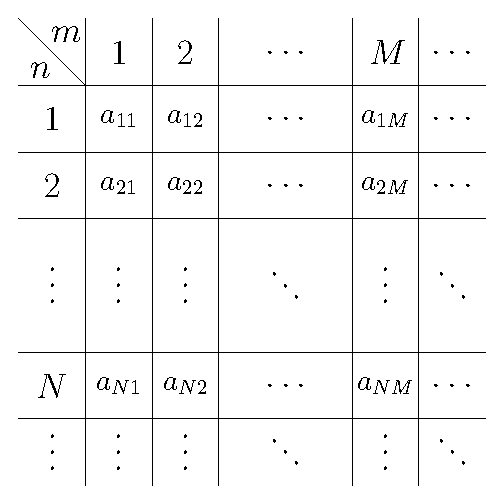
\includegraphics[width=0.3\textwidth]{MA3L16_1.eps}
	\label{MA3L16_1}
	\caption{Последовательность заданная двумя индексами.}
	\label{fig:построение h(x)}
\end{figure}
Такое суммирование принципиально можно понимать тремя способами. Заметим, все эти способы могут приводить к разным ответам и возникнет естественный вопрос, а когда ответ будет один и тот же? То что ответы разные можно легко увидеть из теорем про произведения двух рядов.
\subsection*{(1) Двойной ряд}
\begin{defn}
	\uwave{Двойным рядом} будем называть суммы вида:
	$$
		\ddsum{n,m = 1}{\infty}a_{nm} = \lim\limits_{\substack{n \to \infty\\ m \to \infty}}\ddsum{i = 1}{n}\ddsum{j = 1}{m}a_{ij} = S
	$$
\end{defn}
\begin{defn}
	\uwave{Частичная сумма двойного ряда} $S_{NM} = \displaystyle \sum\limits_{n \leq N}\sum\limits_{m \leq M} a_{nm}$. 
\end{defn}
\begin{defn}
	Двойной ряд \uwave{сходится} если $\exists \, \lim\limits_{\substack{N \to \infty\\ M \to \infty}} S_{NM}$, этот предел называется \uwave{суммой} и равен $S$.
\end{defn}

\begin{rem}
	Напоминание из прошлого семестра (см. семинары):
	$$
		\lim\limits_{\substack{N \to \infty\\ M \to \infty}} S_{NM} = S \Leftrightarrow \forall \VE > 0, \, \exists \, K \colon \forall N,M \in \MN \colon N > K, M > K, \, |S_{NM} - S| < \VE
	$$
	Это тоже самое, что и предел $\lim\limits_{\substack{x \to \infty\\ y \to \infty}}f(x,y)$.
\end{rem}

\begin{prop}
	Если двойной ряд $\displaystyle\sum\limits_{n,m = 1}^{\infty}a_{nm}$ сходится, то $\lim\limits_{\substack{n \to \infty\\ m \to \infty}}a_{nm} = 0$.
\end{prop}
\begin{proof}
	Распишем член ряда через его частичные суммы:
	$$
		a_{nm} = S_{nm} - S_{n-1 m} - S_{n m - 1} + S_{n -1 m - 1 }  \to S - S - S + S = 0
	$$
\end{proof}

Заметим, что если задана последовательность $a_{nm}$, то также имеем последовательность частичных сумм и наоборот, если задана последовательность частичных сумм, то можно восстановить последовательность $a_{nm}$. Для простого ряда было:
$$
	S_n = a_1 + a_2 + \dotsc + a_n \Leftrightarrow a_n = S_n - S_{n-1}
$$
Соответственно, в нашем случае ситуация следующая:
$$
	S_{nm} = \ddsum{i = 1}{n}\ddsum{j = 1}{m}a_{nm} \Leftrightarrow a_{nm} = S_{nm} - S_{n-1m} - S_{nm-1} + S_{n-1m-1}
$$
\begin{rem}
	Из того, что $a_{nm} \to 0$ не следует, что $a_{nm}$ - ограничена. Более того, из сходимости ряда этого тоже не следует. Это так, поскольку стремление к нулю говорит про $n,m > K$, но ничего не говорит про то, что происходит с $a_{n1}$ или $a_{1m}$, например:
	$$
		a_{1m} = m, \, a_{2m} = -m, \, \forall k > 2, \, a_{km} = 0 \Rightarrow \sum\limits_{\substack{n \leq N\\ m \leq M}}a_{nm} = 0
	$$
\end{rem}

\begin{theorem}
	Двойной ряд с положительными членами $a_{nm} \geq 0$ сходится тогда и только тогда, когда его частичные суммы ограничены.
\end{theorem}
\begin{proof}
	Очевидно, что если ряд сходится, то его частичные суммы - ограничены. Пусть $S_{NM} \leq L$ и обозначим точную верхнюю грань по всем таким суммам $S = \sup\limits_{N,M}\{S_{NM}\}$. Покажем, что $S$ будет являться суммой ряда. Пусть $\VE > 0$, тогда:
	$$
		\exists \, S_{N_0 M_0} \colon  S_{N_0 M_0} > S - \VE \Rightarrow \forall n > N_0, m > M_0, \, S_{nm} > S - \VE
	$$
	где последнее очевидно: $S_{nm} \leq S_{kp}, \, \forall n \leq k, m \leq p$, поскольку члены ряда неотрицательны. Тогда:
	$$
		\forall \VE > 0, \, \exists \, N_0, M_0 \colon \forall n > N_0, m > M_0, \, |S_{nm} - S| < \VE
	$$
	Это и означает, что: $S = \lim\limits_{\substack{n \to \infty\\ m \to \infty}}S_{nm}$.
\end{proof}

\begin{theorem}
	Если сходится двойной ряд из абсолютных значений данного ряда, то и сам ряд сходится.
\end{theorem}
\begin{proof}
	Пусть $a_{nm} = b_{nm} + c_{nm} = \max\{a_{nm},0\} - \min\{0, a_{nm}\}$, тогда очевидно, что: 
	$$
		0 \leq b_{nm} \leq |a_{nm}|, \, 0 \leq c_{nm} \leq |a_{nm}|
	$$
	Таким образом, из сходимости двойного ряда из абсолютных значений следует ограниченность сумм и соответственно сходимость рядов:
	$$
		\ddsum{n,m = 1}{\infty}b_{nm}, \, \ddsum{n,m = 1}{\infty}c_{nm}
	$$
	Следовательно сходится и их сумма равная исходному ряду:
	$$
		\ddsum{n,m = 1}{\infty}a_{nm} = \ddsum{n,m = 1}{\infty}b_{nm} + \ddsum{n,m = 1}{\infty}c_{nm}
	$$
\end{proof}

\subsection*{(2) Повторные ряды}
\begin{defn}
	\uwave{Повторными рядами} будем называть суммы вида:
	$$
		\ddsum{n = 1}{\infty}\left(\ddsum{m = 1}{\infty}a_{nm}\right) = \lim\limits_{N \to \infty}\left(\lim\limits_{M \to \infty} S_{NM}\right) \text{ или }\ddsum{m = 1}{\infty}\left(\ddsum{n = 1}{\infty}a_{nm}\right) = \lim\limits_{M \to \infty}\left(\lim\limits_{N \to \infty} S_{NM}\right)
	$$
\end{defn}
\begin{rem}
	То есть эти суммы это просто повторные пределы. Из семинаров прошлого семестра известно, что это совсем не тоже самое, что и двойной предел. Заметим также, что повторное суммирование это разные способы суммирования. В одном может быть сходимость, а в другом её может не быть вовсе.
\end{rem}
\begin{defn}
	Повторный ряд \uwave{сходится}, если сходятся все ряды по индексу $m$ и их суммы равны $S_n$:
	$$
		\forall n, \, \ddsum{m = 1}{\infty}a_{nm} = S_n
	$$
	и если сходится ряд из этих сумм:
	$$
		\ddsum{n = 1}{\infty}S_n = \ddsum{n = 1}{\infty}\ddsum{m = 1}{\infty}a_{nm}
	$$
\end{defn}
\begin{rem}
	Аналогично сходимость определяется для суммирования сначала по $n$, затем по $m$.
\end{rem}
Здесь также можно применить теорему про совпадение двойного ряда и повторного, аналогичную теореме про совпадение повторного предела и двойного предела (см. лекция $9$, курс $2$).
\begin{theorem}
	Если сходится двойной ряд $\ddsum{n,m = 1}{\infty}a_{nm}$ и сходятся все ряды по индексу $m$, то сходится и повторный ряд и имеет ту же сумму, что и двойной ряд:
	$$
		\ddsum{n,m = 1}{\infty}a_{nm} = S = \ddsum{n = 1}{\infty}\ddsum{m = 1}{\infty}a_{nm}
	$$
\end{theorem}
\begin{proof}
	Следует напрямую из теоремы о равенстве двойного предела и повторных.
\end{proof}
\begin{rem}
	Теорема аналогично может быть сформулирована для суммирования по индексу $n$.
\end{rem}
\subsection*{(3) Простые ряды}
\begin{defn}
	\uwave{Простыми рядами} будем называть суммы вида:
	$$
		\ddsum{k = 1}{\infty}a_{n(k)m(k)}
	$$
	где $k \mapsto (n(k), m(k))$ - биекция, которая нумерует все клетки таблицы.
\end{defn}

\begin{theorem}
	Пусть даны двойной и простой ряды, состоящие из одних и тех же членов. Тогда абсолютная сходимость одного из них влечет абсолютную сходимость другого и равенство их сумм.
\end{theorem}
\begin{proof}
	Пусть сходится абсолютно двойной ряд, тогда будет верно:
	$$
		\ddsum{n,m = 1}{\infty}|a_{nm}| = S
	$$
	Возьмем частичную сумму простого ряда модулей:
	$$
		\forall K, \, \ddsum{k = 1}{K}|a_{n(k)m(k)}| \leq \ddsum{n,m = 1}{\infty}|a_{nm}| = S
	$$
	Следовательно простой ряд абсолютно сходится. Пусть теперь сходится абсолютно простой ряд:
	$$
		\ddsum{k = 1}{\infty}|a_{n(k)m(k)}| = A
	$$
	тогда для любой частичной суммы абсолютного двойного ряда:
	$$
		\ddsum{n = 1}{N}\ddsum{m = 1}{M}|a_{nm}| = S_{NM}
	$$
	Следовательно, $\exists \, K$ такое, что все слагаемые этой суммы будут содержаться среди первых $K$ членов простого абсолютного ряда и тогда: $S_{NM} < A$. В этом случае, двойной ряд будет сходиться абсолютно. 
	
	Поскольку простой ряд сходится абсолютно, то в нём мы можем переставить слагаемые любым биективным способом (см. лекцию $4$) $\Rightarrow$ расположим их по ``квадратам'' (т.е. на схеме идем от левого верхнего угла к правому нижнему растущими квадратами), тогда возьмем частичную сумму по целому квадрату:
	$$
		A = \lim\limits_{N \to \infty}\ddsum{n = 1}{N}\ddsum{m = 1}{N}a_{nm} = \lim\limits_{N = M \to \infty} S_{NN} = S
	$$
\end{proof}
\newpage
\subsection*{Сходимость двойных, повторных и простых рядов}
Рассмотрим несколько примеров.

\textbf{Пример}: $S_{NM} = \dfrac{1}{N}\sin{M} + \dfrac{1}{M}\sin{N}$, тогда:
$$
	\forall N, \, \nexists \, \lim\limits_{M \to \infty} S_{NM},\, \forall M, \, \nexists \, \lim\limits_{N\to \infty} S_{NM}
$$
Но при этом существует двойной предел:
$$
	\exists \, \lim\limits_{\substack{N \to \infty \\ M \to \infty}} S_{NM} = 0
$$

Таким образом, заметим, что следующие пределы - разные и по смыслу, и по значению:
$$
	\lim\limits_{N \to \infty}\left(\lim\limits_{M \to \infty} S_{NM}\right), \, \lim\limits_{M \to \infty}\left(\lim\limits_{N \to \infty} S_{NM}\right), \, \lim\limits_{\substack{N \to \infty \\ M \to \infty}} S_{NM}
$$

\textbf{Пример}: $S_{NM} = \dfrac{NM}{N^2 + M^2}$, тогда:
$$
	\lim\limits_{N \to \infty}\left(\lim\limits_{M \to \infty} S_{NM}\right) = \lim\limits_{N \to \infty}\left(0\right) = 0
$$
Но при этом, если мы возьмем $N = M$:
$$
	S_{NN} = \dfrac{N^2}{N^2 + N^2} = \dfrac{1}{2} \nrightarrow 0
$$
То есть не существует двойного предела:
$$
	\forall \VE > 0, \, \exists \, K \colon \forall N > K, M > K, \, |S_{NM} - S| < \VE
$$
$$
	N = M \to \infty \Rightarrow S = \dfrac{1}{2}; \, M > K, \, N \to \infty \Rightarrow S = 0
$$
\begin{theorem}
	Если хотя бы один из рядов:
	$$
		\ddsum{n,m = 1}{\infty}a_{nm},\, \ddsum{n = 1}{\infty}\left(\ddsum{m = 1}{\infty}a_{nm}\right), \, \ddsum{m = 1}{\infty}\left(\ddsum{n = 1}{\infty}a_{nm}\right), \, \ddsum{k = 1}{\infty}a_{n(k)m(k)}
	$$
	сходится абсолютно, то все ряды сходятся абсолютно и их суммы равны.
\end{theorem}
\begin{proof}
	Пусть сходится ряд $\ddsum{k = 1}{\infty}|a_{n(k)m(k)}|$ и его сумма равна $S$. Тогда $\forall N ,m, \, \ddsum{n = 1}{N}|a_{nm}|\leq S$. Следовательно ряд сходится абсолютно и сходится ряд $\ddsum{n = 1}{\infty}a_{nm}$ для любых $m$. По определению:
	$$
		\forall \VE > 0 ,\, \exists \, K \colon \forall k > K, \, \ddsum{k = K + 1}{\infty}|a_{n(k)m(k)}| < \VE \Rightarrow \left|\ddsum{k = K + 1}{\infty}a_{n(k)m(k)}\right| = \left|S - \ddsum{k =  1}{K}a_{n(k)m(k)} \right| < \VE
	$$
	При больших $N$ и $M$, следующая разность есть сумма группы членов $a_{n(k)m(k)}$ для номеров с $k > K$:
	$$
		\exists \, N_0, M_0 \colon \forall N > N_0, M > M_0, \, \left|\ddsum{m = 1}{M}\ddsum{n = 1}{N}a_{nm} - \ddsum{k = 1}{K}a_{n(k)m(k)}\right| \leq \ddsum{k = K + 1}{\infty}|a_{n(k)m(k)}| < \VE
	$$
	Перейдем к пределу по $N \to \infty$, поскольку ряд по $n$ сходится, то:
	$$
		\forall M > M_0, \, \left|\ddsum{m = 1}{M}S_m - \ddsum{k = 1}{K}a_{n(k)m(k)}\right| \leq \VE 
	$$
	Тогда мы получим:
	$$
		\forall M > M_0, \,\left|\ddsum{m = 1}{M}S_m - S\right| \leq \left|\ddsum{m = 1}{M}S_m - \ddsum{k = 1}{K}a_{n(k)m(k)}\right|  + \left| \ddsum{k =  1}{K}a_{n(k)m(k)} - S \right| < 2\VE
	$$
	Следовательно, повторный ряд сходится к $S$. Наоборот, если сходится ряд  $\ddsum{m = 1}{\infty}\left(\ddsum{n = 1}{\infty}|a_{nm}|\right) =S$, то:
	$$
		\forall N, M, \, \ddsum{m = 1}{M}\left(\ddsum{n = 1}{N}|a_{nm}|\right) < S
	$$
	Рассмотрим частичную сумму простого ряда от $1$ до $K$, тогда:
	$$
		\forall K, \, \exists \, N_0, M_0 \colon \forall N > N_0, M > M_0, \, \ddsum{k = 1}{K}|a_{n(k)m(k)}| \leq \ddsum{m = 1}{M}\left(\ddsum{n = 1}{N}|a_{nm}|\right) < S
	$$
	Следовательно, простой ряд сходится абсолютно $\Rightarrow$ сходится. Аналогичное утверждение в обе стороны будет верно для повторной суммы сначала по $m$ и затем по $n$. Объединяя это с теоремой про равенство абсолютной сходимости простого и двойного рядов мы получаем требуемое.
\end{proof}

\begin{exrc}
	Исследовать сходимость ряда:
	$$
		\ddsum{n,m = 0}{\infty}\dfrac{1}{n^p + m^p}, \, p > 0
	$$
\end{exrc}

\newpage
\section*{Кратные степенные ряды}
Пусть последовательность задана двумя индексами $\{c_{nm}\}_{n,m = 1}^{\infty}$, будем рассматривать следующий кратный степенной ряд (предварительно сделав сдвиг по переменным в $z_0 = 0$, $w_0 = 0$):
$$
	\ddsum{n,m = 0}{\infty}c_{nm}z^n w^n, \, \forall n,m, \, c_{nm} \in \MC,\, z,w \in \MC
$$
Область сходимости этого ряда не обязана представлять из себя что-то обобщающее круг сходимости. Иногда можно переписать этот ряд в виде повторного:
$$
	\ddsum{n = 0}{\infty}\left(\ddsum{m = 0}{\infty}c_{nm}w^m\right)z^n
$$
Но это тогда просто степенной ряд по переменной $z$ и аналогично по $w$, где радиусы сходимости будут зависеть от другой переменной: $|z| \leq R(w)$ и $|w| \leq R(z)$. Таким образом, область сходимости не обязательно будет выглядеть как прямоугольник: $|z| < R, \, |w| < R_1$, более того, область сходимости может не содержать внутренних точек. Но можно ли понять, что этот ряд где-то сходится?
\begin{prop}
	Предположим, что $z_1 \neq 0, \, w_1 \neq 0$ и $\exists \, M \colon \forall n,m, \, |c_{nm}z_1^n w_1^m| \leq M$. Тогда $\forall q \in (0,1)$ на области:
	$$
		\{(z,w)\colon |z| \leq q|z_1|, \, |w| \leq q|w_1|\}
	$$
	степенной ряд $\ddsum{n,m = 0}{\infty}c_{nm}z^n w^n$ сходится абсолютно и равномерно.
\end{prop}
\begin{proof}
	Поскольку $|z| \leq q|z_1|$ и $|w| \leq q|w_1|$, тогда:
	$$
		|c_{nm}z^n w^m| \leq |c_{nm}z_1 w_1|q^n q^m \leq M q^{n + m}
	$$
	Рассмотрим следующий ряд с неотрицательными слагаемыми:
	$$
		\ddsum{n,m = 0}{\infty}q^{n+m}
	$$
	Из теоремы про сходимость кратных рядов достаточно исследовать на сходимость один из трех известных рядов. Рассмотрим повторный ряд, поскольку все слагаемые неотрицательны, то:
	$$
		\ddsum{n = 0}{\infty}\left(\ddsum{m = 0}{\infty}q^{n + m}\right) = \ddsum{ n = 0}{\infty}\dfrac{q^n}{1-q} = \dfrac{1}{(1-q)^2} < \infty \Rightarrow \ddsum{n,m = 0}{\infty}q^{n+m} < \infty 
	$$
	Обозначим частичную сумму кратного степенного ряда следующим образом:
	$$
		S_{NK}(z,w) = \ddsum{n = 0}{N}\ddsum{m = 0}{K}c_{nm}z^n w^m
	$$
	Равномерная сходимость означает то же самое, что и всегда:
	$$
		S_{NK} \uconv{E} S \Leftrightarrow \sup\limits_{(z,w) \in E}\left|S_{NK}(z,w) - S(z,w)\right| \xrightarrow[N,K \to \infty]{} 0
	$$
	Тогда:
	$$
		\left|S_{NK}(z,w) - S(z,w)\right| = \left|\ddsum{\substack{n = N + 1 \\ m  = K + 1}}{\infty} c_{nm}z^n w^m \right| \leq M{\cdot}\ddsum{\substack{n = N + 1 \\ m  = K + 1}}{\infty}q^{n + m} \to 0
	$$
	Поскольку хвост у сходящегося ряда стремится к нулю, то взяв супремум, мы получим требуемое.
\end{proof}
\begin{rem}
	Рассматриваем $\{(z,w) \colon |z| \leq q|z_1| \wedge |w| \leq q|w_1|\}$, где $(z_1,w_1)$ взяты из утверждения. Тогда ряд:
	$$
		\ddsum{n,m = 0}{\infty}|c_{nm}|{\cdot}|z|^n{\cdot}|w|^m
	$$
	сходится. Следовательно, по теореме о равенстве кратных сходящихся рядов, мы можем рассматривать исходный ряд в следующем виде:
	$$
		\ddsum{n,m = 0}{\infty}c_{nm}z^n w^m = \ddsum{n = 0}{\infty}\left(\ddsum{m = 0}{\infty}c_{nm} z^nw^m\right) = \ddsum{n = 0}{\infty}\left(\ddsum{m = 0}{\infty}c_{nm} w^m\right)z^n = f(z,w)
	$$
	Всё свелось к одномерному случаю. При фиксированном $w$ получим степенной ряд по $z$ и наоборот $\Rightarrow$ можно применять весь инструментарий из обычных степенных рядов. В частности, можно дифференцировать бесконечное число раз на множестве сходимости (можно считать почленно дифференцируя):
	$$
		\exists \, \dfrac{\partial^{n + m}f}{\partial z^n \partial w^m}(z,w)
	$$
	И, в частности, если взять такую производную в нуле, мы получим коэффициенты ряда:
	$$
		\dfrac{\partial^{n + m}f}{\partial z^n \partial w^m}(0,0) = c_{nm} n! m!
	$$
	Следовательно, этот ряд окажется рядом Тейлора для своей суммы, только понадобится сделать группировку по степеням $n$ и $m$, чтобы порядок производной был один и тот же, тогда это получится в чистом виде дифференциал.
\end{rem}

\textbf{Пример}: Пусть $z_1 \neq 0$ и $c_{0m} = z_1 m!, \, c_{1m} = -m!, \, \forall k \geq 2,\, c_{km} = 0$, $N \geq 2$. Тогда:
$$
	S_{NK} = \ddsum{n = 0}{N}\ddsum{m = 0}{K}c_{nm}z^n w^m = \ddsum{m = 0}{K}w^m \left(z - z_1\right)m!
$$
Этот ряд сходится $\Leftrightarrow w = 0$ или $z = z_1$. Никаких внутренних точек сходимости нет.
\begin{rem}
	В учебнике Фихтенгольца теорема Абеля для кратных степенных рядов формулируется с ошибкой. Там отсутствует требование ограниченности и делается ошибочный вывод, что из сходимости следует ограниченность коэффициентов.
\end{rem}
Таким образом, для кратных степенных рядов, если в какой-то точке установили, что слагаемые ограничены, то появлется разумная область сходимости с которой уже можно работать. В том числе, сводится всё к повторным рядам и анализируются, как обычные степенные ряды, в противном случае, всё становится очень сложным.
\newpage
\textbf{Пример}: Рассмотрим следующий ряд:
$$
	\ddsum{n,m = 0}{\infty}C_{n + m}^n z^n w^m
$$ 
Найти область сходимости? Рассмотрим область, где этот ряд сходится абсолютно:
$$
	\ddsum{n,m = 0}{\infty}C_{n + m}^n {\cdot}|z|^n{\cdot} |w|^m = \ddsum{k = 0}{\infty}\ddsum{n,m \colon n + m = k}{}C_{n + m}^n {\cdot}|z|^n{\cdot}|w|^m = \ddsum{k = 0}{\infty}\left(|z| + |w|\right)^k = \dfrac{1}{1 - (|z| + |w|)}
$$
Таким образом, ряд сходится при $|z| + |w| < 1$. Внутри этого ромба ряд сходится, вне - расходится, что происходит на границе области - вопрос.

\end{document}